\section{Procedure}\label{sec:procedure}
A waveguide was constructed in \mefisto{} and filled with two dielectric media, as shown in Fig.~\ref{fig:waveguide}.

\begin{figure}[tbph]
	\centering
	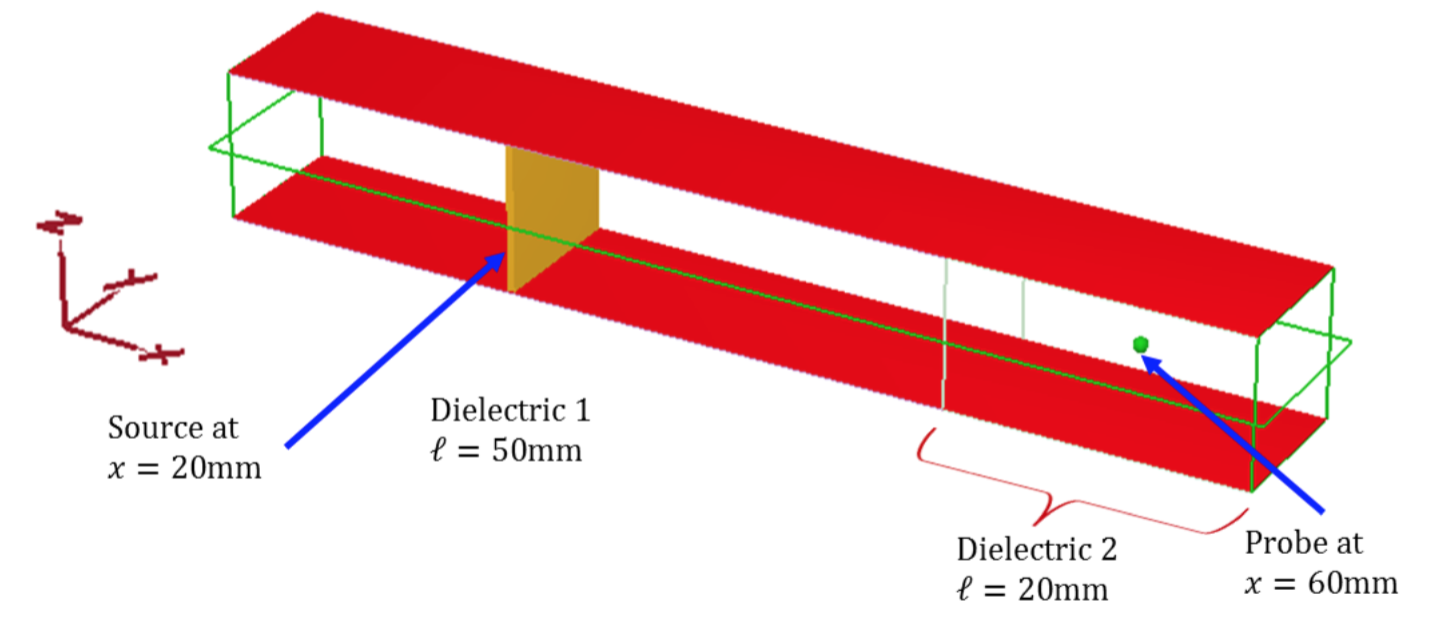
\includegraphics[width=0.7\linewidth]{graphics/waveguide}
	\caption{Parallel plate waveguide}
	\label{fig:waveguide}
\end{figure}

Initially, we made both dielectrics identical and changed the right end to a perfect electrical boundary.
The source generated a 10 GHz plane wave through the structure.
By observing the wave envelope in the structure we were able to determine the standing wave amplitudes, $E_{max} $and $E_{min}$, and positions of $l_{max}$ and $l_{min}$.
The type of right boundary (absorbing, electric, magnetic) was changed, as well as the dielectric properties $\epsilon_r$ and $\sigma$.
See Section~\ref{sec:discussion} for the effect of these variations of the wave patterns.

\pagebreak 
 
A third material was added to study the use of dielectrics as impedance transformers.
The structure is shown in Fig.~\ref{fig:waveguide_3dielectrics}

\begin{figure}[tbph]
	\centering
	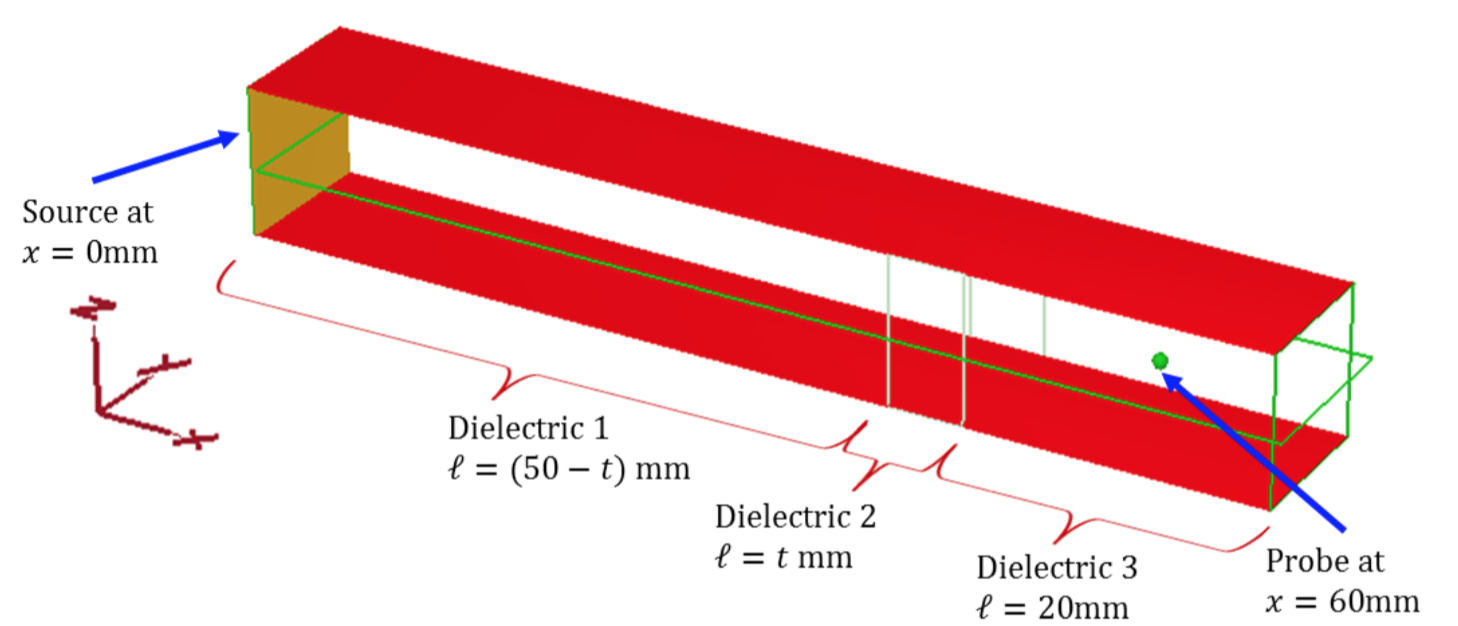
\includegraphics[width=0.7\linewidth]{graphics/waveguide_3dielectrics}
	\caption{Waveguide with three dielectric regions}
	\label{fig:waveguide_3dielectrics}
\end{figure}

By choosing the length of the second dielectric region as $\sfrac{\lambda_2}{4}$ and $\epsilon_2 = \sqrt{\epsilon_1 \epsilon_3}$, we were able to create several impedance transformers by varying the length of the second medium and by using different pairs of input frequency and medium size.
